\let\negmedspace\undefined
\let\negthickspace\undefined
\documentclass[journal]{IEEEtran}
\usepackage[a5paper, margin=10mm, onecolumn]{geometry}
%\usepackage{lmodern} % Ensure lmodern is loaded for pdflatex
\usepackage{tfrupee} % Include tfrupee package

\setlength{\headheight}{1cm} % Set the height of the header box
\setlength{\headsep}{0mm}     % Set the distance between the header box and the top of the text

\usepackage{gvv-book}
\usepackage{gvv}
\usepackage{cite}
\usepackage{amsmath,amssymb,amsfonts,amsthm}
\usepackage{algorithmic}
\usepackage{graphicx}
\usepackage{textcomp}
\usepackage{xcolor}
\usepackage{txfonts}
\usepackage{listings}
\usepackage{enumitem}
\usepackage{mathtools}
\usepackage{gensymb}
\usepackage{comment}
\usepackage[breaklinks=true]{hyperref}
\usepackage{tkz-euclide} 
\usepackage{listings}
% \usepackage{gvv}                                        
\def\inputGnumericTable{}                                 
\usepackage[latin1]{inputenc}                                
\usepackage{color}                                            
\usepackage{array}                                            
\usepackage{longtable}                                       
\usepackage{calc}                                             
\usepackage{multirow}                                         
\usepackage{hhline}                                           
\usepackage{ifthen}                                           
\usepackage{lscape}
\usepackage{circuitikz}
\tikzstyle{block} = [rectangle, draw, fill=blue!20, 
    text width=4em, text centered, rounded corners, minimum height=3em]
\tikzstyle{sum} = [draw, fill=blue!10, circle, minimum size=1cm, node distance=1.5cm]
\tikzstyle{input} = [coordinate]
\tikzstyle{output} = [coordinate]


\begin{document}

\bibliographystyle{IEEEtran}
\vspace{3cm}

\title{9-9.6-5}
\author{EE24BTECH11063 - Y. Harsha Vardhan Reddy}
 \maketitle
% \newpage
% \bigskip
{\let\newpage\relax\maketitle}

\renewcommand{\thefigure}{\theenumi}
\renewcommand{\thetable}{\theenumi}
\setlength{\intextsep}{10pt} % Space between text and floats


\numberwithin{equation}{enumi}
\numberwithin{figure}{enumi}
\renewcommand{\thetable}{\theenumi}

\textbf{Question}:\\
For the following differential equation, find the general solution satisfying the given condition:\\
$$\cos^2{x}\frac{dy}{dx}+y=\tan{x} \brak{0\le x\le\frac{\pi}{2}}$$\\
\solution \\
First let us solve the given differential equation theoritically and then do it computationally and verify if they are equal \\
\begin{align}
   \cos^2{x}\frac{dy}{dx}+y=\tan{x}
\end{align}
or \begin{align}
    \frac{dy}{dx} + \sec^2{x}\cdot y= \sec^2{x}\cdot \tan{x}
\end{align}
Integrating factor,
\begin{align}
    e^{\int{sec^2{x}}\cdot dx}=e^{\tan{x}}
\end{align}
By multiplying integrating factor on both sides
\begin{align}
    \int{d(e^{\tan{x}}\cdot y)}=\int{e^{\tan{x}}. \sec^2{x}\cdot \tan{x}dx}
\end{align}
\begin{align}
e^{\tan{x}}\cdot y=e^{\tan{x}}\brak{\tan{x}-1} + c
\end{align}
(where c is constant of integration)\\
Let us verify our solution for $x=1$ and $y=1$\\
By substituting $x=1$ and $y=1$,\begin{align}
    c=e^{\tan{1}}\cdot \brak{2-\tan{1}}
\end{align}
Final equation,
\begin{align}
    e^{\tan{x}}\cdot y=e^{\tan{x}}\brak{\tan{x}-1} + e^{\tan{1}}\cdot \brak{2-\tan{1}}
\end{align}
Now let us verify this computationally
From definition of $\frac{dy}{dx}$,
\begin{align}
    y_{n+1}=y_{n}+\frac{dy}{dx}\cdot h    
\end{align}
(where h is small number tending to zero)
From the differential equation given,
\begin{align}
    \frac{dy}{dx}=\frac{\tan(x)-y}{\cos^2{x}}
\end{align}
By substituting,
\begin{align}
    y_{n+1}=y_{n}+\brak{\frac{\tan(x_n)-y_n}{\cos^2{x_n}}}\cdot h
\end{align}
By taking $x_1=0 \text{ and } y_1=1.10076$  and $h=0.04$ going till $x=2$ by iterating through the loop and finding $y_2,y_3,\cdots , y_{500}$ and plotting the graph the implicit function we can verify if the function we got by solving the differential equation mathematically.
The comparision between theoretical and simulated graphs is shown in the following page ~\ref{fig:1}\\
Clearly, both theoretical and simulated curves are coinciding and Hence the theoretical solution is verified.
\begin{figure}[ht]
    \centering
    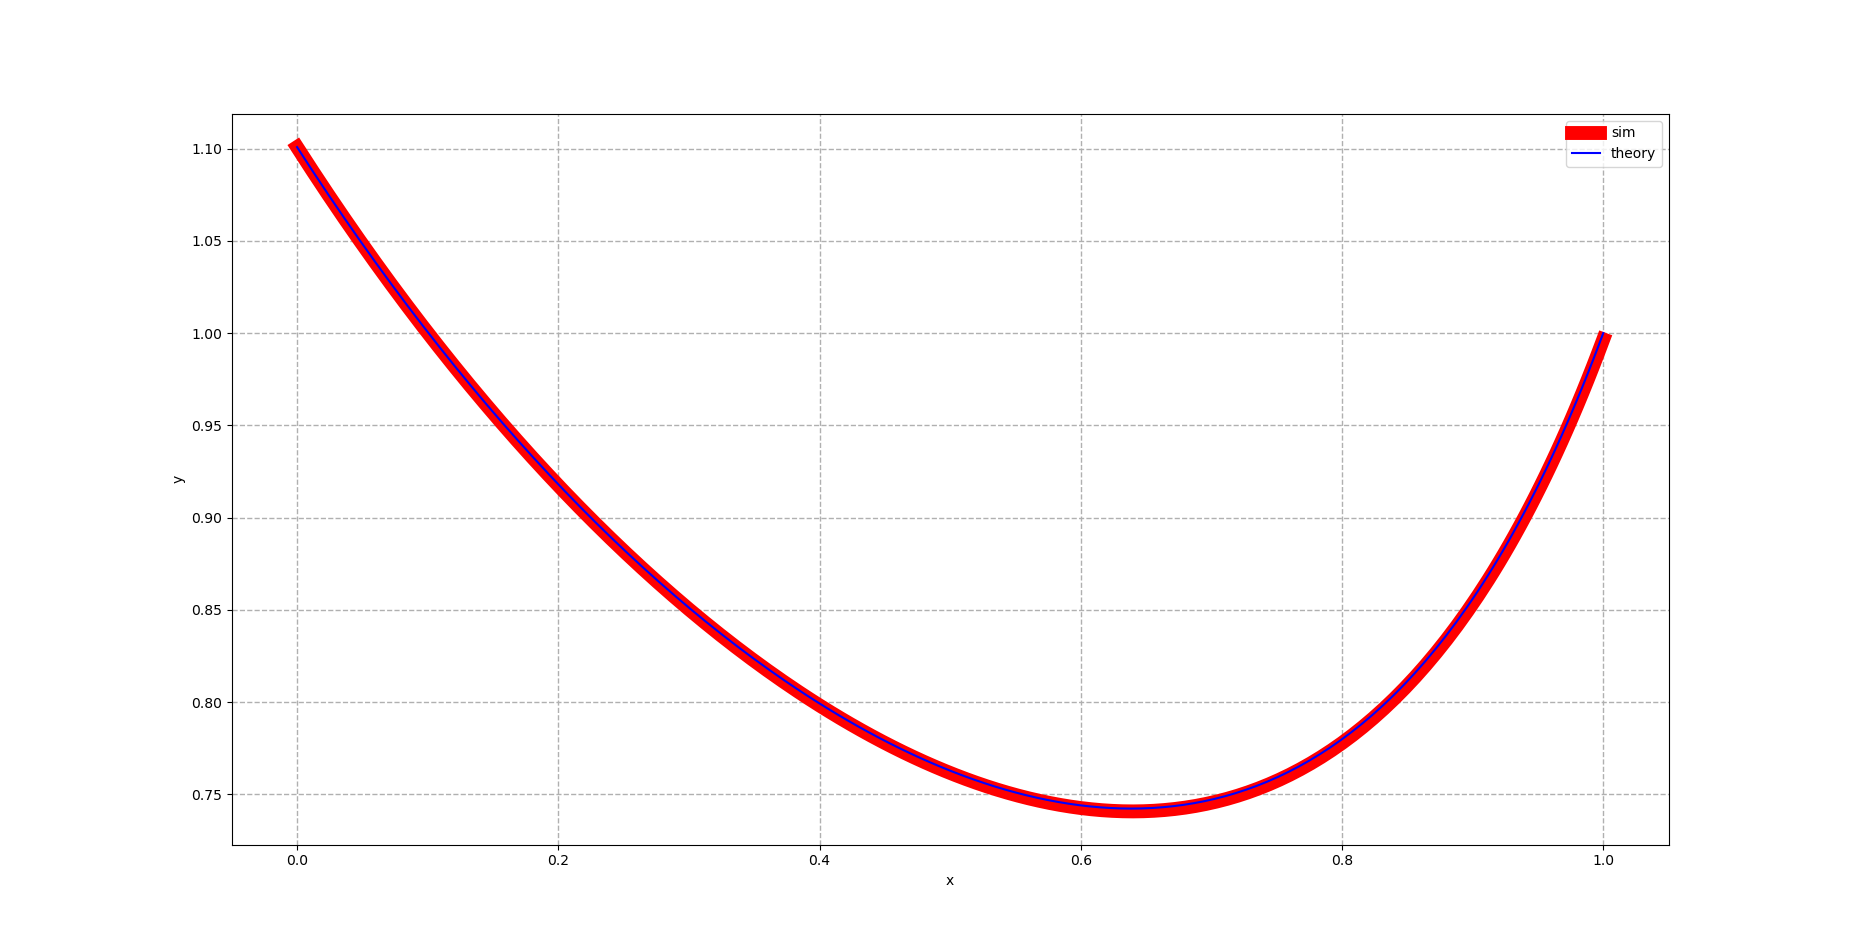
\includegraphics[width=\columnwidth]{figs/Figure_1.png}
    \caption{}
    \label{fig:1}
\end{figure}
\end{document}





